%----------------------------------------------------------------------------------------
%	PART 1: Dasar Pemrograman
%----------------------------------------------------------------------------------------
\part{PEMROGRAMAN PYTHON}

%\chapterimage{head1.png} % Chapter heading image
\chapter{PENDAHULUAN}
\setcounter{page}{1}
\pagenumbering{arabic}
%----------------------------------------------------------------------------------------
%	Mengubah halaman dari romawi menjadi arabic
%----------------------------------------------------------------------------------------
\section{Apa itu Program?}
Program merupakan kumpulan perintah dari manusia kepada komputer untuk melakukan  suatu tugas tertentu. Biasanya suatu program tidak berdiri tunggal melainkan tersusun dalam desain tertentu untuk membentuk suatu perangkat lunak (\textit{software}). Menurut fungsinya perangkat lunak dibedakan menjadi 3 kategori :

\begin{enumerate}
	\item \textit{Perangkat lunak sistem}, perangkat lunak yang bertanggung jawab dalam memanajemen komponen perangkat keras (\textit{hardware}). Contohnya adalah sistem operasi, kernel, driver dlsb.
	\item \textit{Perangkat lunak programming}, perangkat lunak yang digunakan programer untuk menulis program. Contohnya adalah \textit{text-editor}, compiler, intrepreter, linker, debugger (biasanya telah menjadi sebuah satu-kesatuan perangkat lunak yang disebut dengan \textit{Integrated Development Environtment} (IDE)). Contohnya Netbeans, Pycharm, Anaconda, Eclipse dlsb.
	\item \textit{Perangkat lunak aplikasi}, perangkat lunak yang digunakan untuk melakukan tugas tertentu. Contohnya MS. Office yang digunakan untuk membantu proses bisnis kantoran, Google Chrome yang digunakan untuk browsing internet, dlsb.
\end{enumerate}

\section{Bahasa Pemrograman}
\begin{figure}[hbt!]
    \centering
    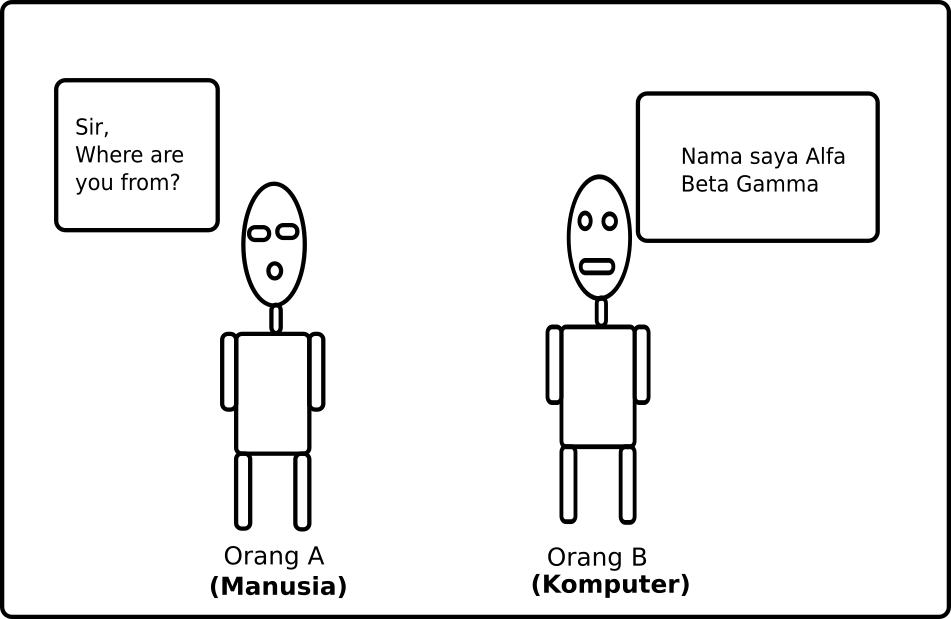
\includegraphics[width=.7\textwidth]{61_comp.png}
    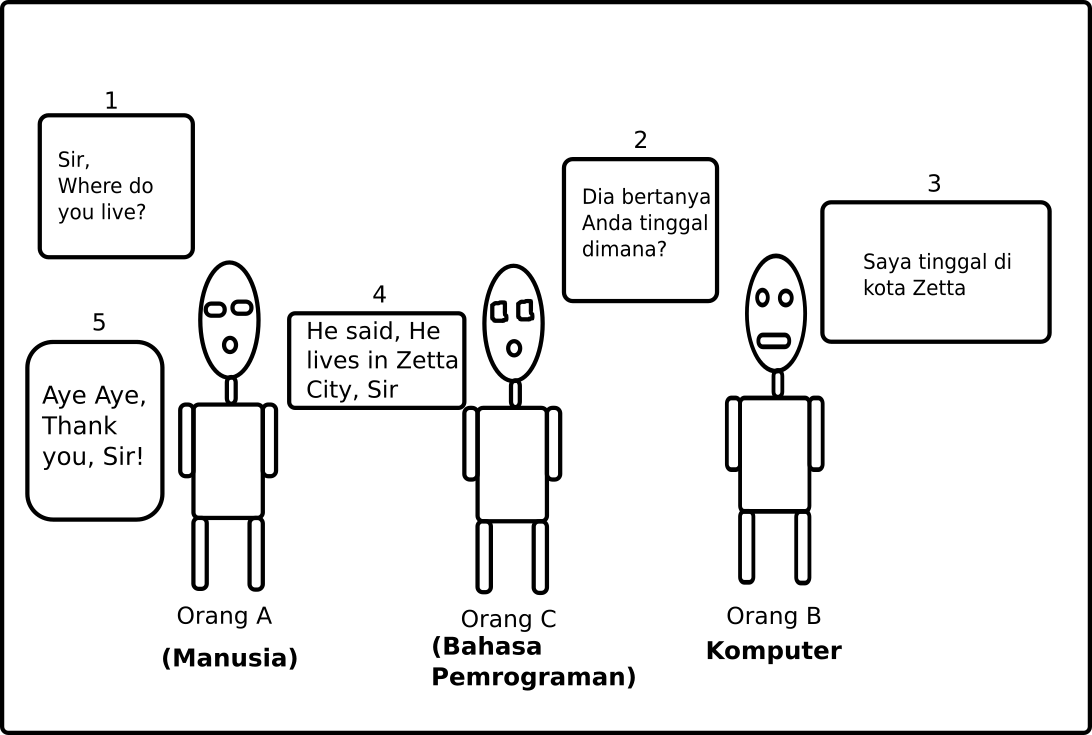
\includegraphics[width=.7\textwidth]{62_comp1.png}
    \caption{(Atas) Komunikasi 2 orang berbeda warga negara (orang A dan orang B) sebagai abstraksi komunikasi antara manusia dengan komputer. (Bawah) Komunikasi 2 orang berbeda warga negara (orang A dan orang B) kemudian ditengai oleh seorang translator (Orang C) \emph{(Gambar ini dirancang dan digambar oleh penulis)}}
    \label{fig:61_comp}
	\end{figure}

Komputer tidak bisa menulis program. Komputer juga tidak mengerti bahasa manusia. Disinilah letak peranan dari bahasa pemrograman, yaitu sebagai jembatan komunikasi antara manusia dengan komputer. Untuk abstraksi yang lebih jelas terkait dengan peranan bahasa pemrograman dapat Anda amati pada gambar (\ref{fig:61_comp}). 

Pada gambar tersebut (gambar atas) tedapat 2 orang yang berbeda warga negara (Orang A dan orang B) yang sedang mencoba berkomunikasi. Namun, karena menggunakan bahasa yang berbeda dapat dipastikan akan terjadi miskomunikasi. Permasalahan ini dapat diatasi apabila Anda bisa mengundang orang ketiga (orang C) sebagai \textit{translator} yang menghubungkan komunikasi antara orang A dan orang B. 

Kedua orang yang ingin berkomunikasi dapat dibayangkan sebagai manusia yang ingin memberikan instruksi pada komputer. Tentu saja, manusia tidak bisa secara langsung memberikan instruksi pada komputer. Itulah sebabnya bahasa pemrograman diciptakan yaitu untuk memberikan jembatan komunikasi antara manusia dan komputer. 

Dari sini bisa didefinisikan bahwa bahasa pemrograman adalah bahasa yang digunakan untuk berkomunikasi dengan komputer. Menurut tingkatannya, bahasa pemrograman dapat dibedakan menjadi 3 kategori yaitu :
\begin{itemize}
	\item Bahasa mesin
	\item Bahasa assembly
	\item Bahasa tingkat tinggi
\end{itemize}

\subsection{Bahasa Mesin}
 Pada gambar (\ref{fig:61_comp}) disebutkan bahwa mesin dibayangkan dapat berkomunikasi dengan sesama mesin dengan menggunakan suatu bahasa tertentu. Bahasa itulah yang dimaksud dengan bahasa mesin. Bahasa mesin (kode mesin) merupakan bahasa tingkat rendah yang secara langsung dikonstruksi dan hanya diperuntukan untuk mesin. Disebut "tingkat rendah" karena konfigurasi kodenya bisa berbeda-beda untuk setiap mesin/platform. Bahasa mesin terdiri atas 2 buah nilai saja : \texttt{0} dan \texttt{1} (sehingga membentuk sistem binary), yang mana biasanya membentuk kelompok byte (8 bit). Berikut adalah contoh dari pada struktur bahasa mesin :

\begin{verbatim}
    01010101 11011011 11110010
\end{verbatim}

Mempelajari bahasa mesin bisa diibaratkan seperti mempelajari bahasa manusia purba\footnote{\textit{Homo Erectus} misalnya}. Karena kebudayaan manusia purba masih rendah tentu sistem bahasa manusia purba tidak memiliki struktur bahasa yang lazim. Sehingga bahasa tersebut sangat susah untuk diartikan dan dipelajari oleh orang manusia modern\footnote{baca "kita"}. Hanya orang-orang tertentu yang bisa mengerti (mempelajari) sistem bahasa manusia purba\footnote{Sejarahwan atau Arkeolog}. 

Mirip dengan itu, bahasa mesin sangat susah untuk dipelajari. Mengapa? Karena untuk pengaplikasiannya, Anda harus mempelajari terlebih dahulu bagaimana struktur dari konstruksi mesin yang dibangun (mengingat bahasa mesin merupakan bahasa yang tergantung oleh arsitektur mesin). Selain itu, penulisan format binary tentu tidak lazim bagi orang modern seperti kita. Dibandingkan dengan jenis bahasa pemrograman yang lain, bahasa mesin memiliki beberapa kelebihan dan kekurangan.

Kelebihan dari bahasa mesin :
\begin{itemize}
	\item Cepat, karena bahasa mesin dieksekusi secara langsung oleh mesin 
	\item Penggunaan memori yang efisien
\end{itemize}

Kekurangan dari bahasa mesin :
\begin{itemize}
	\item Tidak bisa dimengerti oleh manusia (hanya terdiri dari digit \texttt{0} dan \texttt{1}).
	\item Jika terjadi kesalahan (\textit{error}) program akan susah untuk memecahkannya.
	\item Tidak ada fungsi matematika yang tersedia.
	\item Manipulasi lokasi memori dilakukan secara langsung, sehingga mmbutuhkan programer yang bisa melakukan pelacakan untuk setiap lokasi memori.
\end{itemize}

\subsection{Bahasa Assembly}
Menggunakan bahasa mesin memang memiliki kelebihan dalam hal kecepatan, namun demikian menggunakan bahasa mesin tentu saja sangat tidak mudah bagi programer karena skrip kode hanya tediri dari 2 digit bilangan saja (\texttt{0} dan \texttt{1}). Maka dari itu, programer yang ingin bekerja dalam ranah pemrograman tingkat rendah (bahasa mesin) biasanya lebih menyenangi untuk menggunakan bahasa Assembly.

Bahasa assembly pada dasarnya menggantikan bentuk digit binary (\texttt{0} dan \texttt{1}) ke dalam simbol alfanumerik \footnote{kombinasi antara huruf alfabet dan angka-angka} dengan tujuan mempermudah bentuk bahasa mesin. Contohnya adalah sebagai berikut :
\begin{verbatim}
    ADD 1,2, result
\end{verbatim}
Program di atas bertujuan untuk melakukan penjumlahan bilangan \texttt{1} dan \texttt{2} kemudian menampilkan hasilnya.

Jika bahasa mesin bisa diibaratkan sebagai bahasa manusia zaman kuno, maka bahasa assembly bisa diibaratkan sebagai bahasa Sanskerta. Bahasa Sanskerta merupakan bahasa kuno namun lebih terbarukan dibandingkan dengan bahasa yang digunakan oleh manusia purba.  Bahasa Sanskerta sudah memiliki struktur bahasa yang valid dan jelas sehingga masih "dimungkinkan" untuk dibaca dan dipelajari. Namun demikian, untuk mempelajarinya Anda harus menguasai sistem penulisan bahasa Sanskerta terlebih dahulu. Hal ini menjadi faktor ketidakpraktisan mengingat budaya kita sudah tidak menggunakan bahasa Sanskerta lagi. 

Mirip dengan itu, mengembangkan suatu perangkat lunak dengan menggunakan bahasa assembly menjadi barang yang bersifat tidak mungkin untuk dilakukan. Dibandingkan dengan jenis bahasa pemrograman yang lain, bahasa Assembly memiliki beberapa kelebihan dan kekurangan.

Kelebihan dari bahasa assembly :
\begin{itemize}
	\item Lebih mudah digunakan dibandingkan bahasa mesin.
	\item Masih tergolong bahasa tingkat rendah, sehingga kurang cocok digunakan seorang pemula.
\end{itemize}

Kekurangan dari bahasa Assembly :
\begin{itemize}
	\item Tidak ada bentuk simbolik pada lokasi memori.
	\item Masih susah untuk digunakan (khususnya orang awam).
	\item Bentuk bahasa Assembly sangat bergantung pada arsitektur dari mesin (platform) yang digunakan. 
\end{itemize}

\subsection{Bahasa Tingkat Tinggi}
Berbeda dengan kedua jenis bahasa pemrograman di atas yang termasuk golongan bahasa pemrograman tingkat rendah, sehingga untuk penggunaannya memerlukan keahlian khusus\footnote{semisal terkait dengan ilmu konstruksi mesin}, untuk kali ini akan dibahas bahasa pemrograman tingkat tinggi. Dibandingkan dengan bahasa tingkat rendah, dengan menggunakan bahasa pemrograman tingkat tinggi Anda lebih dimudahkan. Bahasa tingkat tinggi bisa diibaratkan sebagai bahasa Inggris yang biasa Anda pelajari di sekolah. Bahasa Inggris sudah terkonstruksi secara apik sehingga sangat mudah untuk dipelajari \footnote{mayoritas manusia modern menguasai bahasa inggris}.

Mirip dengan itu, bahasa tingkat tinggi dikonstruksi untuk mempermudah manusia. Penggunaan sistem pembahasaannya lebih mendekati bahasa manusia dibandingkan dengan bahasa mesin. Bahkan, dengan menggunakan bahasa tingkat tinggi, seseorang yang tidak mengerti tentang arsitektur mesin atau sistem binary bisa melakukan mengkonstruksi program (koding). Bahasa tingkat tinggi juga merupakan bahasa pemrograman yang tidak bergantung pada platform tertentu sehingga sebagai konsekuensinya program yang dihasilkan dapat dieksekusi pada mesin yang berbeda. Namun demikian, jenis bahasa pemrograman yang lebih berorientasi kepada bahasa manusia ini membutuhkan suatu penerjemah, agar instruksi yang diberikan oleh manusia bisa dieksekusi oleh komputer. Penerjemah tersebut dapat dilakukan oleh compiler atau interpreter (tergantung dari jenis bahasa pemrogramannya). Dibandingkan dengan jenis bahasa pemrograman yang lain, bahasa tingkat tinggi memiliki beberapa kelebihan dan kekurangan.

Kekurangan dari bahasa tingkat tinggi :
\begin{itemize}
	\item Harus tersedia penerjemah (compiler atau interpreter).
	\item Kecepatan eksekusi lebih rendah jika dibandingan degan bahasa mesin dan bahasa assembly.
\end{itemize}

Kelebihan dari bahasa tingkat tinggi adalah :
\begin{itemize}
	\item Mudah digunakan (biasanya menggunakan Inggris).
	\item Dapat digunakan di berbagai mesin.
	\item Cocok untuk pemula yang memulai belajar bahasa pemrograman.
\end{itemize}

Contoh dari bahasa tingkat tinggi antara lain adalah C, C++, C#, Java, Fortran, Ruby, Perl, Python dlsb. Bahasa pemrograman tersebut dikonstruksi berdasarkan filosofi dan tujuan komputasi tertentu.

\section{Mengapa harus Python?}
Dewasa ini, Python menjadi bahasa pemrograman yang paling ingin dikuasai oleh mayoritas semua orang (terutama dari kalangan programer). Antusiasme tersebut didukung oleh pesatnya perkembangan teknologi Data Sains \footnote{Data Sains adalah ilmu yang mempelajari perilaku data, baik itu data kuantitatif ataupun numerik.}. Pada bidang Data Sains, dibandingkan dengan bahasa pemrograman lainnya, Python memiliki keunggulan tersendiri dalam hal analitik karena tersedianya library NumPy, Pandas dan Matplotlib (sebagai visualisasi data).

Berbicara terkait library, kini telah tersedia berjuta-juta library di Python. Hal tersebut tentu saja akan mempermudah pekerjaan Anda karena Anda tidak diwajibkan lagi untuk membuat program dari awal. Untuk menuliskan program tertentu Anda hanya perlu memanggil fungsi dari suatu library kemudian menerapkan fungsi tersebut ke dalam program yang sedang Anda kembangkan.

Selain itu, Python sangat mudah untuk dipelajari. Jika Anda belum pernah menginjakan kaki di dunia IT (pemrograman khususnya) maka Python merupakan langkah awal yang tepat. Python juga sangat cocok untuk digunakan sebagai media pembelajaran bahasa pemrograman di dunia pendidikan mengingat Python termasuk bahasa pemrograman yang bersifat \textit{open source}. Meskipun Python merupakan bahasa pemrograman yang mudah dipelajari, Python tetap bisa untuk dijadikan basis untuk membangun sistem yang kompleks.

Satu hal lagi yang membuat Python disenangi oleh kalangan penggiat IT. Python memiliki komunitas yang luas. Jika saja Anda mengalami kesulitan belajar, selalu mengalami kesalahan (\texit{error}) dalam pengembangan program Anda, Anda bisa mengunjungi komunitas Python di forum online yang tersebar luas di internet. Contohnya Anda bisa mengunjungi website : \url{https://www.python.org/community/} dan \url{https://www.stackoverflow.com}.

\section{Soal Latihan}
\begin{enumerate}
	\item Buatlah Essay dengan tema "mengapa belajar pemrograman itu penting"!
	\item Di dalam bahasa pemrograman tingkat tinggi terdapat beberapa paradigma (sudut pandang) dalam  penyajian pemecahan masalah. Diantaranya adalah pemrograman \textit{Imperative}, \textit{Logical}, \textit{Functional} dan \textit{Object-Oriented}. Jelaskan perbedaan dari keempat paradigma pemrograman berikut!
	\item Di dalam bahasa tingkat tinggi terdapat 2 jenis penerjemah, Compiler dan Intrepreter. Jelaskan bagaimana 2 penerjemah itu bekerja kemudian bandingkan juga kekurangan dan kelebihannya!
	\item Sebutkan kelebihan dan kekurangan bahasa pemrograman Python dibandingkan bahasa pemrograman yang lainnya!
	\item Jelaskan bagaimana pembuatan alur program sehingga program tersebut dapat digunakan untuk memecahkan suatu masalah?
\end{enumerate}
